% 1993_旧科目组_文科/figures/f1993_old_arts_q27_prism.tex — 1993 年·旧科目组·文科，第 27 题三棱柱
%
% 【来源】`.work/phase4-b18/source/1993旧科目组文.pdf`（SHA-256 c8e57edcf61e754a36e9b5775c40d9277e0c3f45cb0f93b478118c5cb2219f86），第 1 页；
%   内容流逐路径照录，本地坐标 = 页面坐标 − (1029.610,404.940)，1 单位 = 1 TeX pt。
%   线宽 0.398pt；虚线 [2.989 2.989] 0 d。
%
% 标签相对源中心微调：A₁ 左移 1.49pt、B₁ 右上移 (2.5,4.04)pt、C₁ 右上移 (2.2,2.24)pt，避开顶点与边线
% 元素计数：实线 10 段＋虚线 1 段＋6 个标签
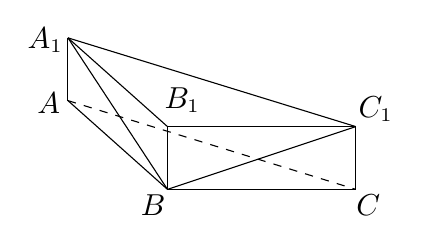
\begin{tikzpicture}[x=1pt, y=1pt,
    every node/.style={inner sep=0pt, font=\fontsize{10.5pt}{12.6pt}\selectfont}]
  \draw[line width=0.398pt] (0.000,32.068) -- (35.968,0.000);
  \draw[line width=0.398pt] (104.005,0.000) -- (35.968,0.000);
  \draw[line width=0.398pt] (0.000,54.747) -- (35.968,22.679);
  \draw[line width=0.398pt] (0.000,54.747) -- (104.005,22.679);
  \draw[line width=0.398pt] (35.968,0.000) -- (35.968,22.679);
  \draw[line width=0.398pt] (0.000,32.068) -- (0.000,54.747);
  \draw[line width=0.398pt] (104.005,22.679) -- (35.968,22.679);
  \draw[line width=0.398pt] (104.005,22.679) -- (35.968,0.000);
  \draw[line width=0.398pt] (0.000,54.747) -- (35.968,0.000);
  \draw[line width=0.398pt] (104.005,22.679) -- (104.005,0.000);
  % 虚线：不可见棱与题设连线
  \draw[line width=0.398pt, dash pattern=on 2.989pt off 2.989pt] (0.000,32.068) -- (104.005,0.000);
  \node[anchor=center] at (-8.200,53.860) {$A_1$};
  \node[anchor=center] at (41.290,32.300) {$B_1$};
  \node[anchor=center] at (111.200,29.000) {$C_1$};
  \node[anchor=center] at (-6.970,31.210) {$A$};
  \node[anchor=center] at (30.770,-5.780) {$B$};
  \node[anchor=center] at (108.560,-5.780) {$C$};
\end{tikzpicture}
%
% 【自验结果】坐标逐点照录内容流；标签取 pdftotext -bbox 中心（字母与下标合并取中点）。
